\clearpage
\subsection{Ultrasonic evaluation}
\begin{figure}
\centering
    \begin{subfigure}[b]{\picwidth}
        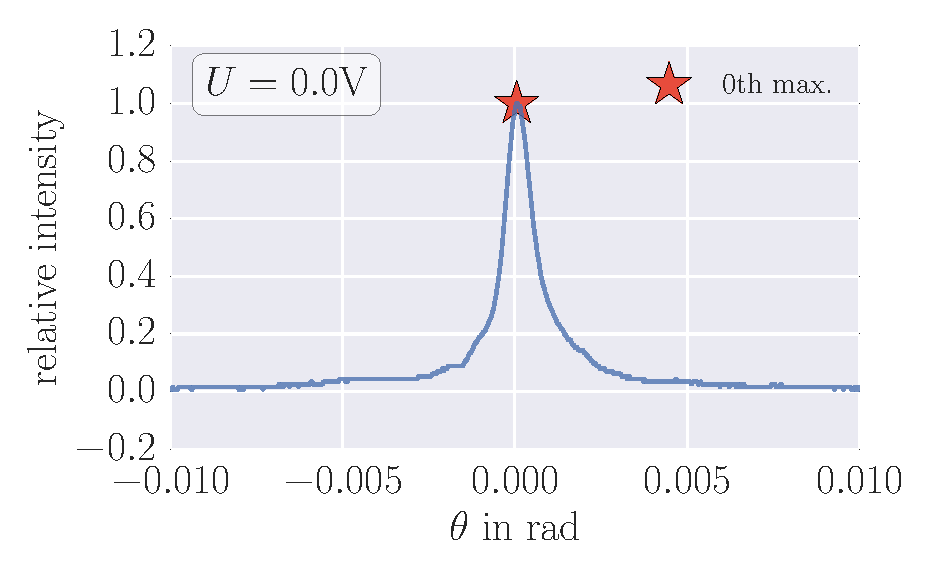
\includegraphics[width=1.0\textwidth]{analysis/figures/raman_001}
        \caption{}
        \label{fig:raman_001}
    \end{subfigure}
    \begin{subfigure}[b]{\picwidth}
        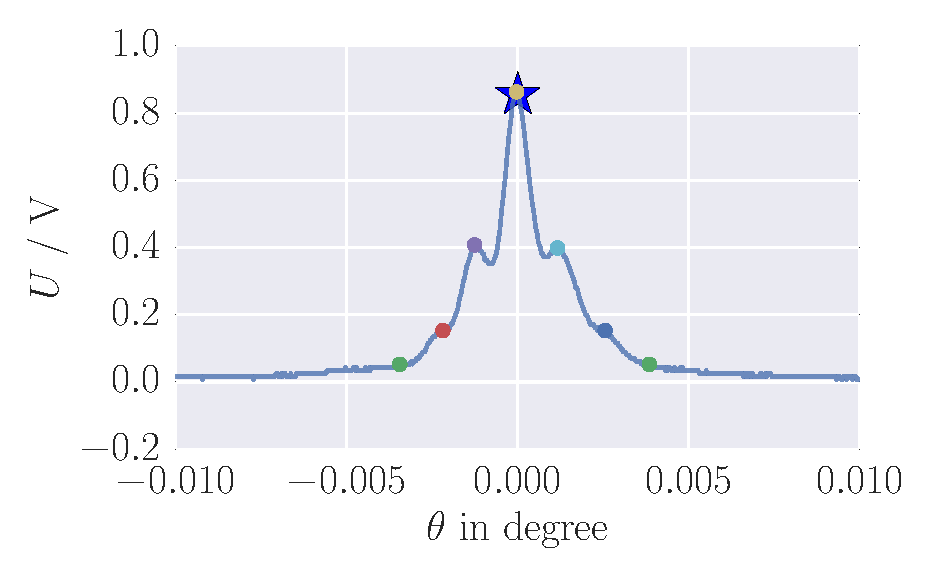
\includegraphics[width=1.0\textwidth]{analysis/figures/raman_007}
        \caption{}
        \label{fig:raman_007}
    \end{subfigure}
    \begin{subfigure}[b]{\picwidth}
        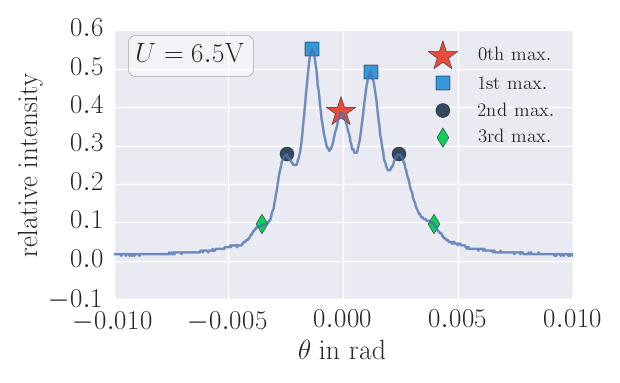
\includegraphics[width=1.0\textwidth]{analysis/figures/raman_014}
        \caption{}
        \label{fig:raman_014}
    \end{subfigure}
    \begin{subfigure}[b]{\picwidth}
        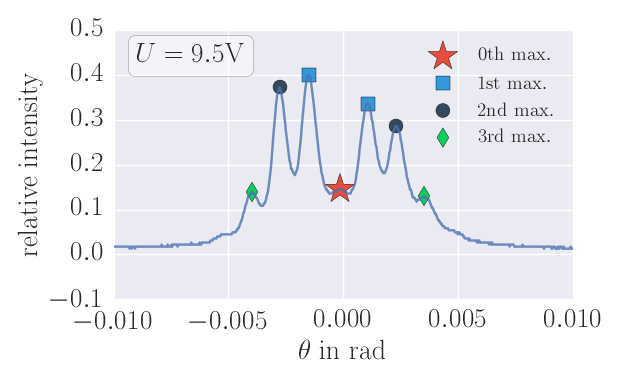
\includegraphics[width=1.0\textwidth]{analysis/figures/raman_020}
        \caption{}
        \label{fig:raman_020}
    \end{subfigure}
    \caption{A subsection of the data from the ultrasonic experiment.}\label{fig:raman}
\end{figure}
\begin{figure}[htpb]
    \centering
    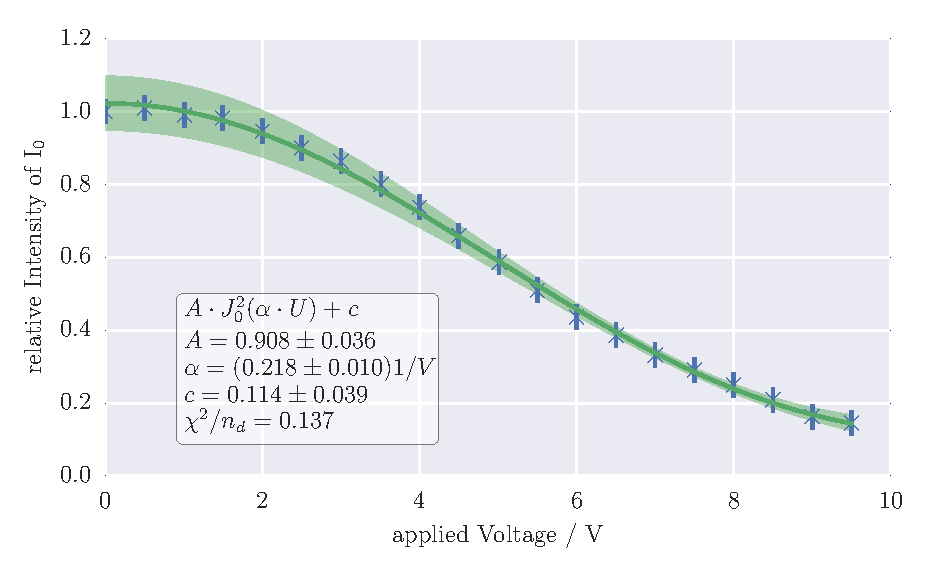
\includegraphics[width=1\textwidth]{analysis/figures/besselfit_000}
    \caption{This is the fit of the maxima of zeroth order. The error is given by 3\% of the extent of the oscilloscope.}
    \label{fig:besselfit_000}
\end{figure}
\begin{SCfigure}
\caption{
BLABLABA
BLABLABA
BLABLABA
BLABLABA
BLABLABA
BLABLABA
BLABLABA
BLABLABA
}
 \begin{tabular}{|r|r|r|r|}
 \hline 
\cellcolor{tabcolor}&\cellcolor{tabcolor}$\alpha$&\cellcolor{tabcolor}$A$&\cellcolor{tabcolor}$c$\\ \hline 
 \cellcolor{tabcolor}$\alpha$&$0.00010$ &$-0.00028$ &$0.00036$ \\ 
\cellcolor{tabcolor}$A$&$-0.00028$ &$0.00132$ &$-0.00130$ \\ 
\cellcolor{tabcolor}$c$&$0.00036$ &$-0.00130$ &$0.00151$ \\ \hline \hline
\cellcolor{tabcolor}$\alpha$&\multicolumn{3}{r|}{$0.21839 \pm 0.00989$ }\\ 
\cellcolor{tabcolor}$A$&\multicolumn{3}{r|}{$0.90833 \pm 0.03628$ }\\ 
\cellcolor{tabcolor}$c$&\multicolumn{3}{r|}{$0.11427 \pm 0.03881$ }\\ 
\hline\end{tabular}
\end{SCfigure}

\clearpage

\begin{figure}[htpb]
    \centering
    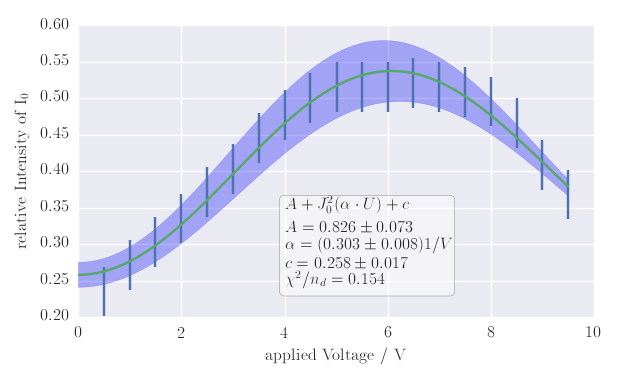
\includegraphics[width=0.8\textwidth]{analysis/figures/besselfit_001}
    \caption{This is the fit of the maxima of zeroth order. The error is given by 3\% of the extent of the oscilloscope.}
    \label{fig:besselfit_001}
\end{figure}


\begin{SCfigure}
\caption{
BLABLABALBALBAL
BLABLABALBALBAL
BLABLABALBALBAL
BLABLABALBALBAL
BLABLABALBALBAL
BLABLABALBALBAL
BLABLABALBALBAL
BLABLABALBALBAL
}
 \begin{tabular}{|r|r|r|r|}
 \hline 
\cellcolor{tabcolor}&\cellcolor{tabcolor}$\alpha$&\cellcolor{tabcolor}$A$&\cellcolor{tabcolor}$c$\\ \hline 
 \cellcolor{tabcolor}$\alpha$&$0.00006$ &$-0.00004$ &$-0.00000$ \\ 
\cellcolor{tabcolor}$A$&$-0.00004$ &$0.00532$ &$-0.00110$ \\ 
\cellcolor{tabcolor}$c$&$-0.00000$ &$-0.00110$ &$0.00029$ \\ \hline \hline
\cellcolor{tabcolor}$\alpha$&\multicolumn{3}{r|}{$0.30305 \pm 0.00792$ }\\ 
\cellcolor{tabcolor}$A$&\multicolumn{3}{r|}{$0.82599 \pm 0.07293$ }\\ 
\cellcolor{tabcolor}$c$&\multicolumn{3}{r|}{$0.25782 \pm 0.01709$ }\\ 
\hline\end{tabular}
\end{SCfigure}
\clearpage
\begin{figure}[htpb]
    \centering
    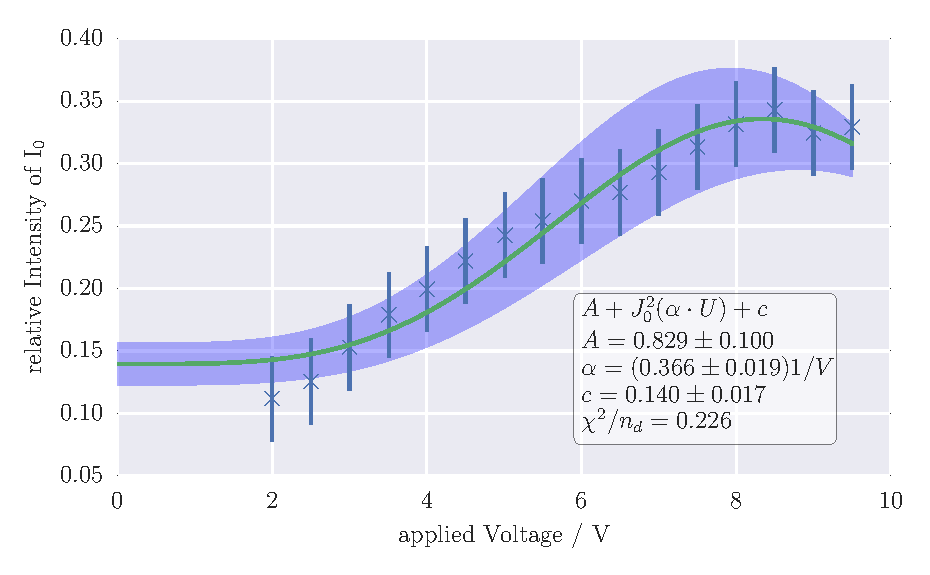
\includegraphics[width=0.8\textwidth]{analysis/figures/besselfit_002}
    \caption{This is the fit of the maxima of zeroth order. The error is given by 3\% of the extent of the oscilloscope.}
    \label{fig:besselfit_001}
\end{figure}

\begin{SCfigure}
\caption{
BLABLABALBLABLABLAB
BLABLABALBLABLABLAB
BLABLABALBLABLABLAB
BLABLABALBLABLABLAB
BLABLABALBLABLABLAB
BLABLABALBLABLABLAB
BLABLABALBLABLABLAB
}
 \begin{tabular}{|r|r|r|r|}
 \hline 
\cellcolor{tabcolor}&\cellcolor{tabcolor}$\alpha$&\cellcolor{tabcolor}$A$&\cellcolor{tabcolor}$c$\\ \hline 
 \cellcolor{tabcolor}$\alpha$&$0.00037$ &$0.00028$ &$-0.00013$ \\ 
\cellcolor{tabcolor}$A$&$0.00028$ &$0.00992$ &$-0.00137$ \\ 
\cellcolor{tabcolor}$c$&$-0.00013$ &$-0.00137$ &$0.00029$ \\ \hline \hline
\cellcolor{tabcolor}$\alpha$&\multicolumn{3}{r|}{$0.36608 \pm 0.01934$ }\\ 
\cellcolor{tabcolor}$A$&\multicolumn{3}{r|}{$0.82888 \pm 0.09961$ }\\ 
\cellcolor{tabcolor}$c$&\multicolumn{3}{r|}{$0.13956 \pm 0.01695$ }\\ 
\hline
\end{tabular}
\end{SCfigure}
\clearpage
\begin{figure}[htpb]
    \centering
    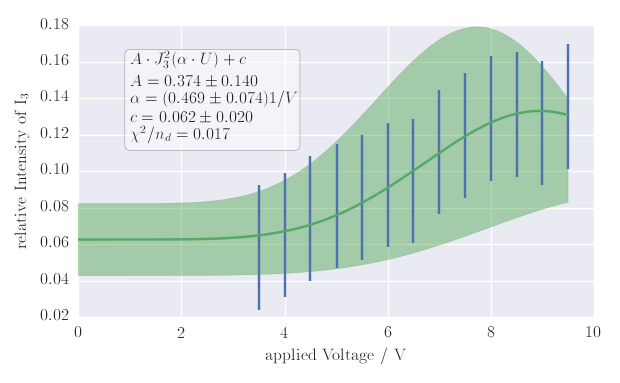
\includegraphics[width=0.8\textwidth]{analysis/figures/besselfit_003}
    \caption{This is the fit of the maxima of zeroth order. The error is given by 3\% of the extent of the oscilloscope.}
    \label{fig:besselfit_001}
\end{figure}
\begin{SCfigure}
\caption{
BLABLABLABLABLASBL
BLABLABLABLABLASBL
BLABLABLABLABLASBL
BLABLABLABLABLASBL
BLABLABLABLABLASBL
BLABLABLABLABLASBL
BLABLABLABLABLASBL
}

 \begin{tabular}{|r|r|r|r|}
 \hline 
\cellcolor{tabcolor}&\cellcolor{tabcolor}$\alpha$&\cellcolor{tabcolor}$A$&\cellcolor{tabcolor}$c$\\ \hline 
 \cellcolor{tabcolor}$\alpha$&$0.00353$ &$-0.00051$ &$-0.00032$ \\ 
\cellcolor{tabcolor}$A$&$-0.00051$ &$0.01381$ &$-0.00112$ \\ 
\cellcolor{tabcolor}$c$&$-0.00032$ &$-0.00112$ &$0.00020$ \\ \hline \hline
\cellcolor{tabcolor}$\alpha$&\multicolumn{3}{r|}{$0.47838 \pm 0.05943$ }\\ 
\cellcolor{tabcolor}$A$&\multicolumn{3}{r|}{$0.40198 \pm 0.11751$ }\\ 
\cellcolor{tabcolor}$c$&\multicolumn{3}{r|}{$0.05726 \pm 0.01415$ }\\ 
\hline\end{tabular}

\end{SCfigure}

